\chapter{Конструкторская часть}

\section{Алгоритм поиска полным перебором в массиве}

На рисунках~\ref{images:full},~\ref{images:generate_perms} представлена схема алгоритма решения задачи коммивояжера полным перебором.

На рисунках~\ref{images:ant_1},~\ref{images:ant_2},~\ref{images:ant_2} представлена схема алгоритма решения задачи коммивояжера муравьиным алгоритмом.


\begin{figure}[H]
    \centering
    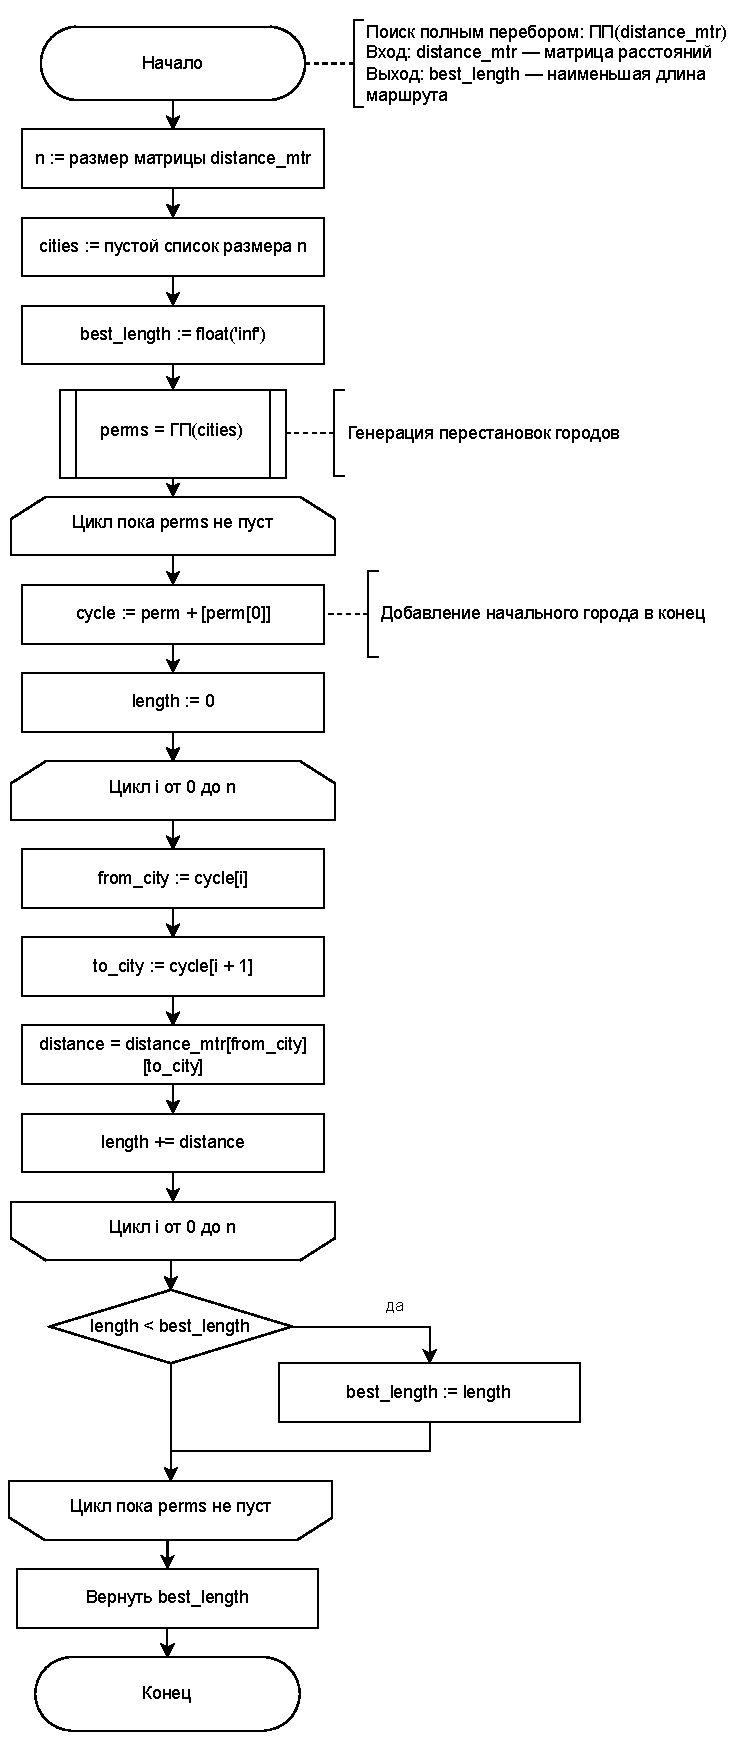
\includegraphics[width=110mm]{images/full}
    \caption{Схема алгоритма решения полным перебором.}
    \label{images:full}
\end{figure}

\begin{figure}[H]
    \centering
    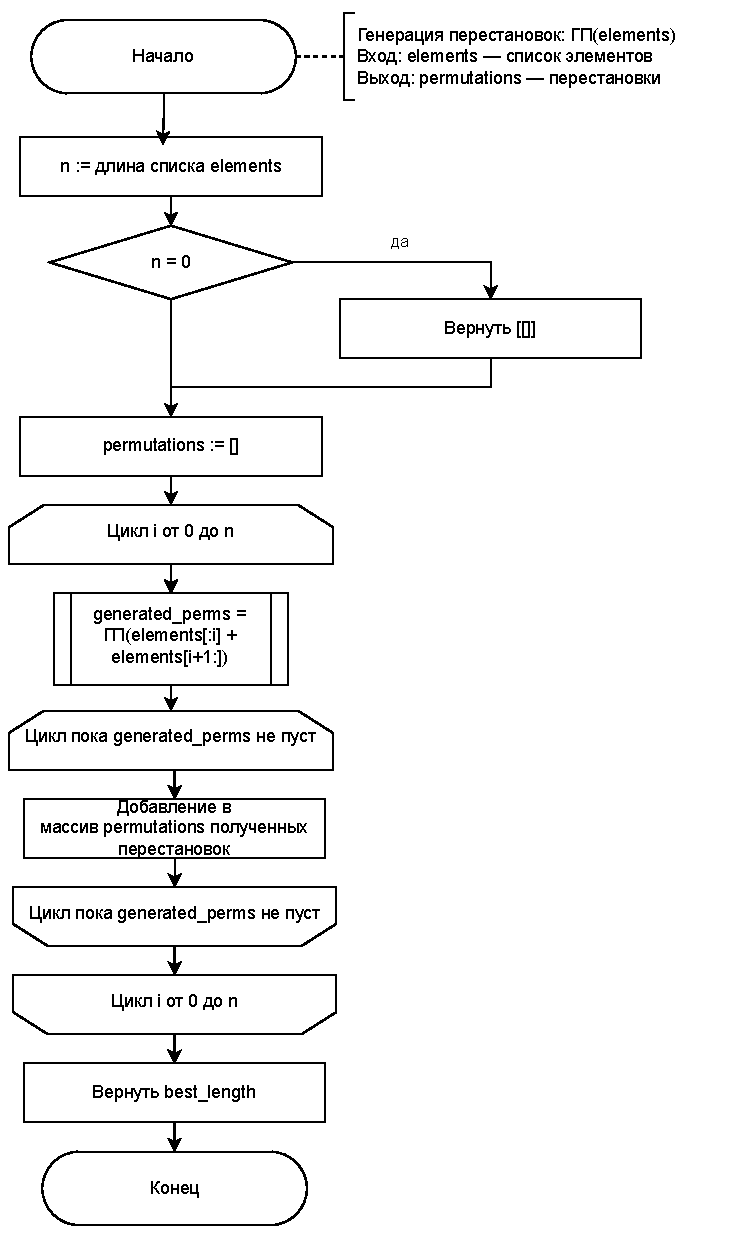
\includegraphics[width=130mm]{images/generate_perms}
    \caption{Схема алгоритма генерации перестановок.}
    \label{images:generate_perms}
\end{figure}


\begin{figure}[H]
    \centering
    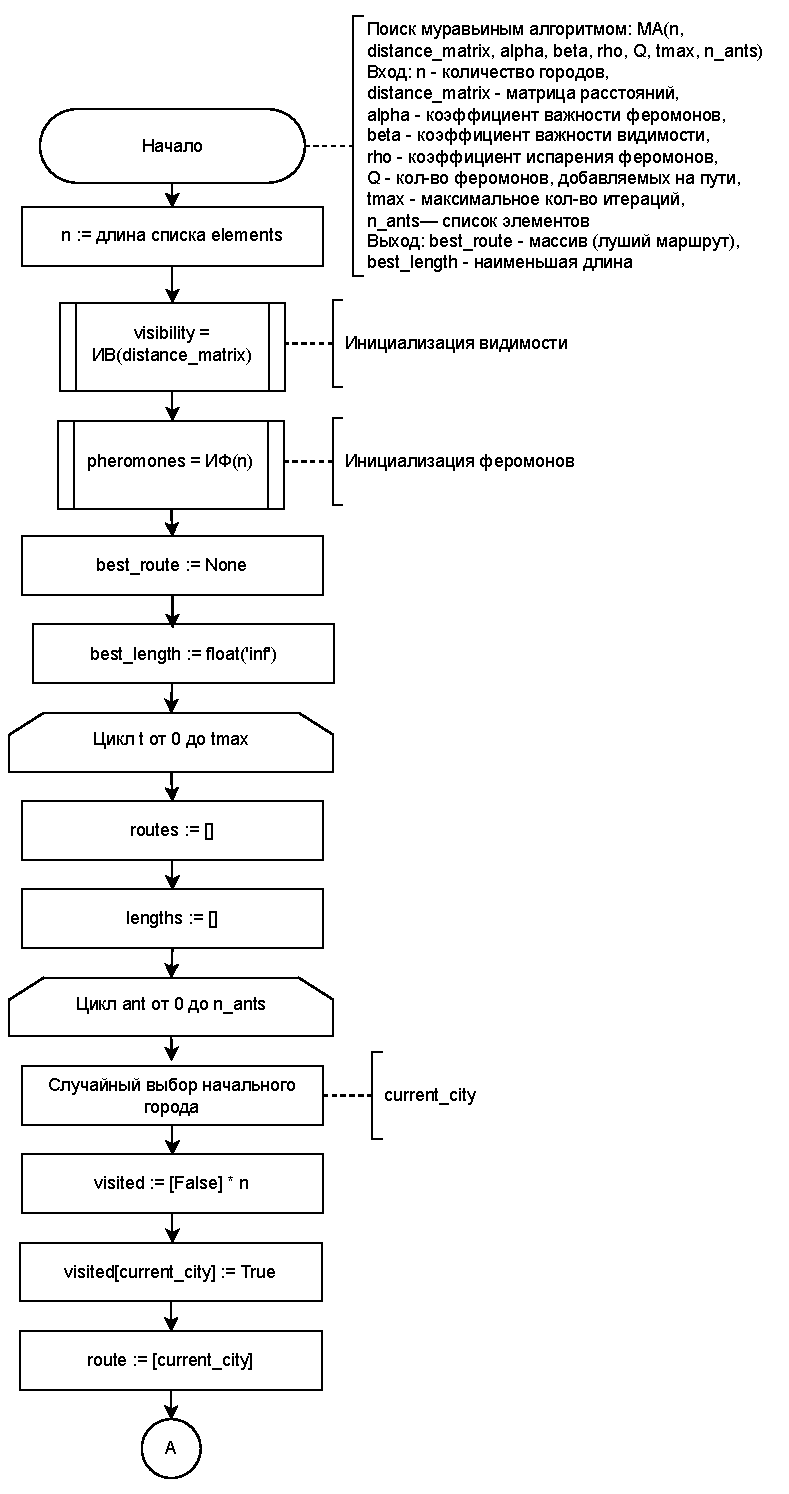
\includegraphics[width=110mm]{images/ant_1}
    \caption{Схема муравьиного алгоритма. Часть 2.}
    \label{images:ant_1}
\end{figure}

\begin{figure}[H]
    \centering
    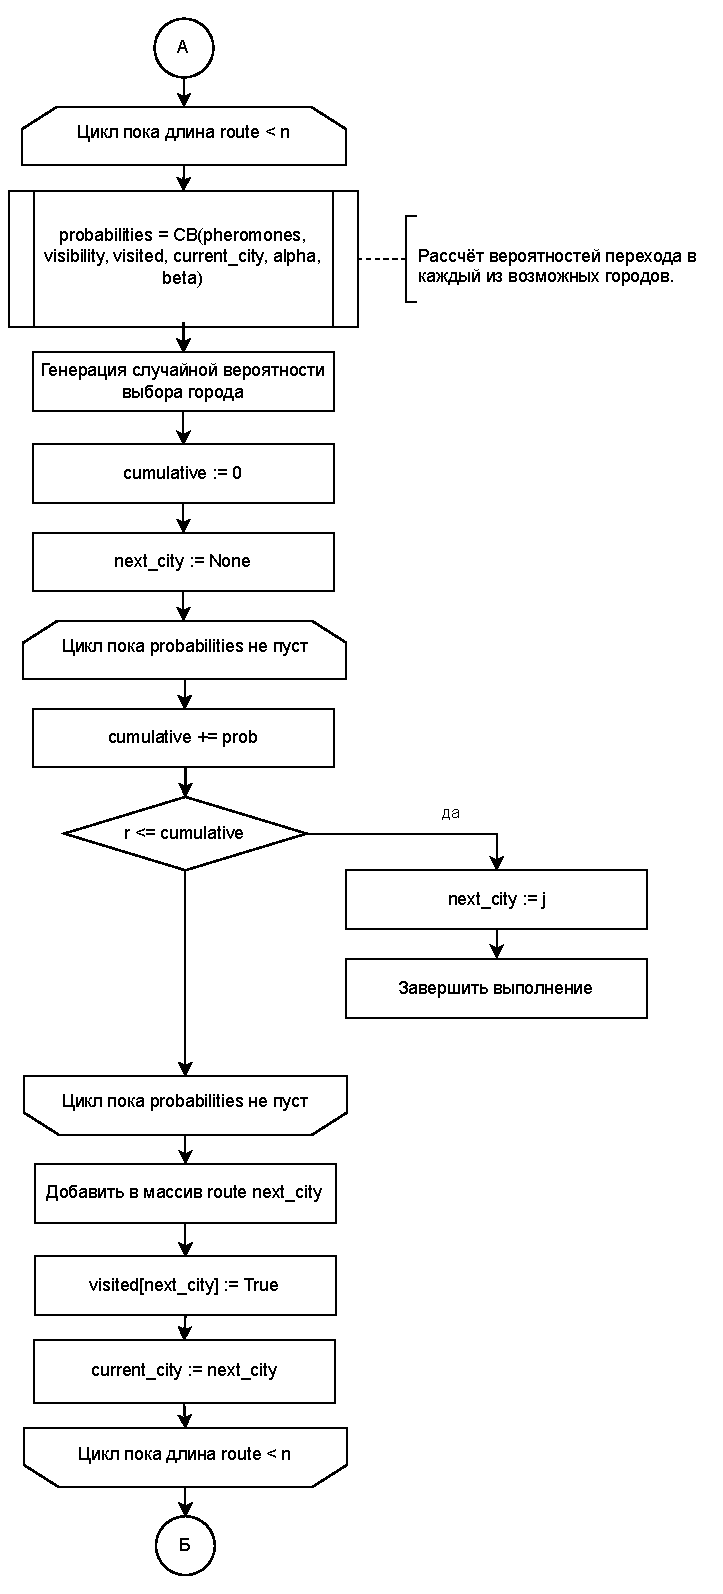
\includegraphics[width=110mm]{images/ant_2}
    \caption{Схема муравьиного алгоритма. Часть 2.}
    \label{images:ant_2}
\end{figure}

\begin{figure}[H]
    \centering
    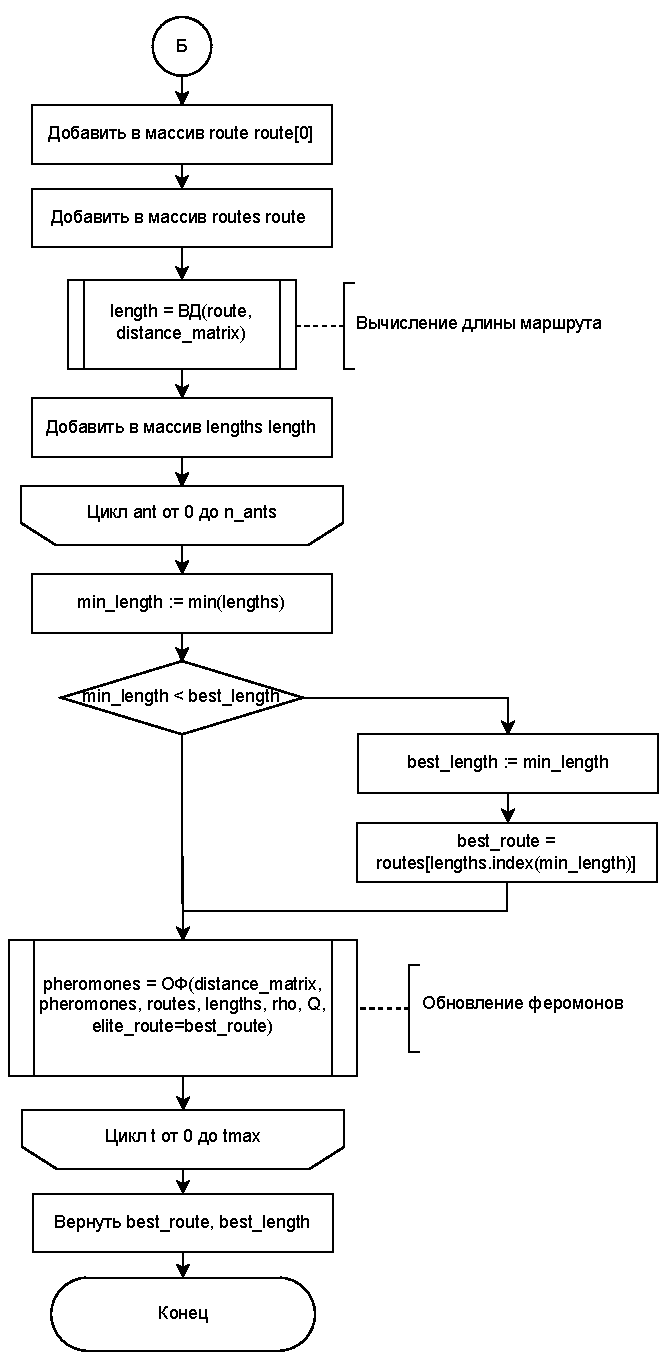
\includegraphics[width=110mm]{images/ant_3}
    \caption{Схема муравьиного алгоритма. Часть 3.}
    \label{images:ant_3}
\end{figure}

\section*{Вывод}

На основе теоретических данных, полученных в аналитическом разделе, были разработаны схемы алгоритмов, необходимых для решения поставленных задач.
